\chapter{Machine Learning and Statistical Physics}
In this introductory chapter, we give an overview of machine learning and its possible applications.
Focusing in particular on one of the most successful models, namely deep neural networks,
we give an introduction to supervised learning problems.

We then move on to establish what connections machine learning has with statistical physics,
altought the former belongs to computer science, while the latter belongs to natural science.
We show the connections between these two disciplines
and give a few examples where the tools of statistical physics can be used to study computer models.

 \section{Machine Learning}
 Machine learning is that branch of artificial intelligence that builds models for machines to learn from data without explicit instructions.
 This field, although it has been studied for several decades, has only recently begun to develop in a prominent way;
 the increase in storage possibilities has increased the amount of data available, which combined with the increase in computing power of computers,
 has led to various application results that were previously difficult to imagine.
 Machine learning algorithms are used in a wide variety of fields, such as medicine, e-mail filtering,
 speech recognition and computer vision, or more generally where it is difficult or impractical to develop conventional algorithms to perform the required tasks.

 One of the most interesting application examples of machine learning is \texttt{GPT-3}~\cite{brown2020language},
 a model based on deep neural networks that can generate content from a description.
 Below is an example where we ask \texttt{GPT-3} to write a paragraph for this thesis;
 we used \href{https://beta.openai.com/playground/}{OpenAI Playground} to interact with the model.
\begin{dialogue}
  \speak{Input} Write a paragraph for my Master's thesis on ``Applying statistical physics to machine learning model''
  \speak{GPT-3} Statistical physics has been shown to be a powerful tool for understanding the behavior of complex systems. In recent years, there has been growing interest in applying statistical physics methods to machine learning models. The goal of this research is to develop a better understanding of how these methods can be used to improve the performance of machine learning models. In particular, we focus on the use of statistical physics methods for analyzing and optimizing the training of neural networks. We believe that this research will lead to a better understanding of the behavior of neural networks and will ultimately improve the performance of machine learning models.
\end{dialogue}

We can divide machine learning techniques into 3 major macro areas, depending on what kind of data is provided to the model to learn:
\begin{itemize}
  \item \emph{supervised learning}: the model is trained using inputs and the corresponding expected outputs, 
                                    it learns from experience;
  \item \emph{unsupervised learning}: the model learns by seeing a collection of samples of the studied distribution;
  \item \emph{reinforcement learning}: the model is allowed to move freely in an environment,
                                       and feedback is provided on the decisions it makes.
\end{itemize}

Machine learning encompasses techniques that come from different branches of mathematics and computer science,
to name a few computational statistics, data mining and image processing.
It is clear that in this context of fast and continuous development,
it is difficult to bring out an overview that can encapsulate and motivate all the empirical rules developed in the field and give them the appropriate theoretical support.

In this work, we will focus on supervised learning with fast-forward deep neural networks.
They are probably the most famous method and on which countless achievements in the discipline are based,
even though even here a complete understanding of how they work is lacking.

\subsection{Supervised learning with deep neural networks}
Deep neural networks were first theorized in the 1950s,
and since then they have undergone countless proposals and tricks to improve their operation.
Here we expose the classic and standard version that came into being when, starting in the 1990s, 
the first applications using them could be had.
Although a modern deep neural network used for a real application has a much more complicated architecture and training algorithm than the one we exhibit,
our model incorporates all the main features without making the problem under consideration any less complex.

To describe a supervised learning process, we must define 3 components:
\begin{itemize}
  \item the data used available for training and a subsequent measure of the goodness of a predictor;
  \item the architecture of the model, with the parameters that define it;
  \item an optimization algorithm that, using the available data, finds the optimal predictor within the chosen architecture.
\end{itemize}
We briefly explain these three components in the case of (deep) neural networks.

\subsubsection{The data}
We assume that we want to train a predictor \(\hat{f}\colon \mathcal{X}\to\mathcal{Y}\),
where \(\mathcal{X}\subseteq\Real^d\) and \(\mathcal{Y}\subseteq\Real\) are called \emph{input space} and \emph{output space} respectively.
The connection between the input and the output is modeled by a joint probability density \(p(\vec{x},y)\);
we assume that the \emph{training set} \(\mathcal{S}\) consists of \(n\) i.i.d. sample of the distribution.

We also need a function that, given a sample, tells us how the predictor is performing on it.
The function \(\loss\colon\mathcal{Y}\times\mathcal{Y}\to\Real^+\) is called the \emph{loss function};
the function wants to emulate a distance in the set \(\mathcal{Y}\), one of the most common choices is \(\loss(y_1,y_2) = (y_1-y_1)^2\).

We also need a way to measure the goodness of a predictor.
The quantity we would like to see minimized is the \emph{theoretical risk}
\[
  \risk_\text{theo} = \E_{p(\vec{x},y)}\left[\loss{(y,\hat{f}{(\vec{x})})}\right],
\]
but it is clearly not accessible, since the distribution of the data is not known.
However, it is possible to have an empirical estimate of risk based on the training set data
\[
  \risk_\text{emp} = \frac{1}{n}\sum_{(\vec{x},y)\in\mathcal{S}}\loss(y,\hat{f}{(\vec{x})}).
\]
Ideally, we would like to find the predictor that minimizes empirical risk.

\subsubsection{The architecture}
Choosing the model architecture is equivalent to defining the \emph{hypothesis class} \(\mathcal{H}\ni\hat{f}\) to where the predictor we want to calibrate belongs.
Selecting as hypothesis classes the set of all functions from \(\mathcal{X}\) to \(\mathcal{Y}\) would certainly result in a predictor such that \(\risk_\text{emp}=0\),
but most likely not able to minimize the loss function on samples out of the training set\footnote{
  For instance, imagine taking a polynomial of a sufficiently high degree to interpolate all points in the training set.
}. The choice of the class of hypotheses is of crucial importance in solving the problem:
we need to have a class of hypotheses large enough to capture all the features of the data distribution,
but still not be specialized to only the training set; in other words, a good class of hypotheses is able to \emph{generalize}
what is learned about the training set even to samples not used for training.
The success of neural networks is due precisely to the fact that they have proven to be an excellent class of hypotheses for problems of application interest (combined with the fact that there are particularly efficient algorithms for training).

Let us start by describing the simplest version of a neural network and,  at the same time, the fundamental component of all networks: the \emph{perceptron}.
The perceptron is a network consisting of a single neuron; it outputs the value of an \emph{activation function}, computed at the biased weighted average of the inputs.
Using formulas
\[
  \hat{f}_{\vec{w},b}{(\vec{x})} = \act{\left(\vec{w}\cdot\vec{x}+b\right)},
\]
where \(\sigma\) is the activation function. The \emph{parameters} of the network are \(\vec{\theta}=(\vec{w},b)\),
they are known as \emph{weight} and \emph{bias} respectively.
Figure~\ref{fig:nn_perceptron} shows a schematic view of a perceptron.
\begin{figure}
  \centering
  \begin{subfigure}{0.495\textwidth}
    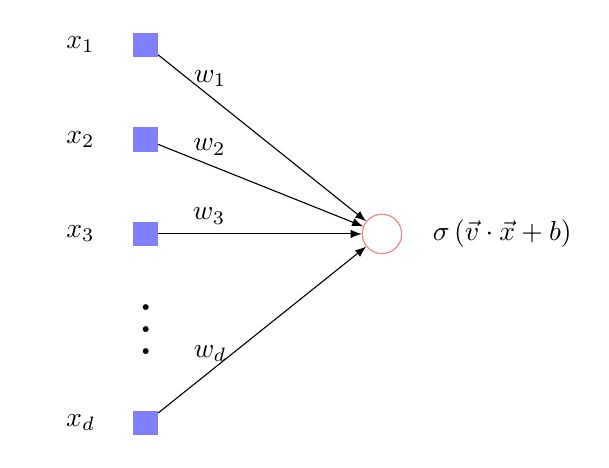
\begin{tikzpicture}[x=1.5cm, y=1.2cm, >=latex]
      \tikzset{
  inputnode/.style={
    rectangle,
    draw,
    minimum size=.3cm
  },
  every neuron/.style={
    circle,
    draw,
    minimum size=.5cm
  },
  neuron missing/.style={
    draw=none, 
    fill=none, %<- added
    scale=2,
    text height=0.333cm,
    execute at begin node=\color{black}$\vdots$
  }
}

\foreach \m [count=\y] in {1,2,3,missing,4} %<- removed "/\l" here 
  \node [fill=black,inputnode/.try, neuron \m/.try,blue!50] (input-\m) at (0,2.5-\y) {};
% added "fill=green" in the line above

\foreach \m [count=\y] in {1}
  \node [every neuron/.try, neuron \m/.try,red!50] (output-\m) at (2,.5-\y) {};

\foreach \l [count=\i] in {1,2,3,d}
  \path (input-\i) -- ++(-1,0)
   node [midway] {$x_\l$};

\foreach \l [count=\i] in {1}
  \path (output-\i) -- ++(1.3,0)
    node [near end] {$\sigma\left(\vec{v}\cdot\vec{x}+b\right)$};

\foreach \i in {1,...,4}
  \foreach \j in {1}
    \draw [->] (input-\i) -- (output-\j);

\foreach \l [count=\i] in {1,2,3,d}
  \foreach \j in {1}
    \path (input-\i) -- (output-\j)
      node [above,near start] {$w_\l$};

% \foreach \l [count=\x from 0] in {Eingangs-, Ausgangs-}
%   \node [align=center, above] at (\x*4,2) {\l \\ Neuronen};
    \end{tikzpicture}
    \caption{perceptron}
    \label{fig:nn_perceptron}
  \end{subfigure}
  \begin{subfigure}{0.495\textwidth}
    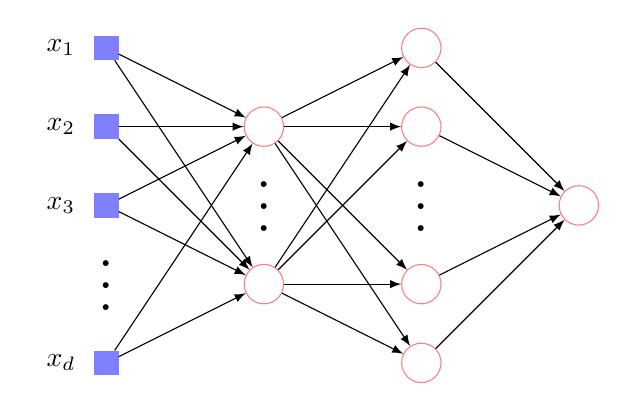
\begin{tikzpicture}[x=1.cm, y=1.cm, >=latex]
      \tikzset{
  inputnode/.style={
    rectangle,
    draw,
    minimum size=.3cm
  },
  every neuron/.style={
    circle,
    draw,
    minimum size=.5cm
  },
  neuron missing/.style={
    draw=none, 
    fill=none, %<- added
    scale=2,
    text height=0.333cm,
    execute at begin node=\color{black}$\vdots$
  }
}

\foreach \m [count=\y] in {1,2,3,missing,4} %<- removed "/\l" here 
  \node [fill=black,inputnode/.try, neuron \m/.try,blue!50] (input-\m) at (0,2.5-\y) {};
% added "fill=green" in the line above

\foreach \m [count=\y] in {1,missing,2}
  \node [every neuron/.try, neuron \m/.try,red!50] (hiddenone-\m) at (2,1.5-\y) {};

\foreach \m [count=\y] in {1,2,missing,3,4}
  \node [every neuron/.try, neuron \m/.try,red!50] (hiddentwo-\m) at (4,2.5-\y) {};

\foreach \m [count=\y] in {1}
  \node [every neuron/.try, neuron \m/.try,red!50] (output-\m) at (6,.5-\y) {};

\foreach \l [count=\i] in {1,2,3,d}
  \path (input-\i) -- ++(-1,0)
   node [midway] {$x_\l$};

% \foreach \l [count=\i] in {1,n}
%   \draw [->] (output-\i) -- ++(1,0)
%    node [above, midway] {$a_\l$};

\foreach \i in {1,...,4}
  \foreach \j in {1,...,2}
   \draw [->] (input-\i) -- (hiddenone-\j);

\foreach \i in {1,...,2}
  \foreach \j in {1,...,4}
    \draw [->] (hiddenone-\i) -- (hiddentwo-\j);

\foreach \i in {1,...,4}
  \foreach \j in {1}
    \draw [->] (hiddentwo-\i) -- (output-\j);

% \foreach \l [count=\x from 0] in {Eingangs-, Ausgangs-}
%   \node [align=center, above] at (\x*4,2) {\l \\ Neuronen};
    \end{tikzpicture}
    \caption{fully connected deep neural network}
    \label{fig:nn_ffnn}
  \end{subfigure}
  \caption{
    schematic view of and perceptron neural networks.
  }
  \label{fig:nn}
\end{figure}
A perceptron can only learn distributions that are linearly separable.

Let's move to the definition of \emph{fast-forward fully connected neural network}.
We can stack neurons in many layers, a neuron takes as input the output of all neurons in the previous layer (the first layer use the input data instead);
the last layer consists of just a neuron whose output is the output of the network.
The topology of the network is defined by the \emph{meta-parameters}: the network will have \(l\) layers with \(f_1,\dots,f_l\) parameters each;
the meta-parameters are fixed before optimization begins and are never changed again.
Writing an explicit formula of the function represented by the neural network is complicated,
it is much more effective to look at the schematic representation in Figure~\ref{fig:nn_ffnn}.
Network parameters are the set of parameters of individual neurons \(\vec{\Theta} = (\vec{\theta}_{1,1},\dots,\vec{\theta}_{l,f_l})\).

Several variants to this construction can be considered (networks not fully connected, different activation functions, parameters shared by multiple neurons, etc.),
but we limit ourselves to this one since for the theoretical approach they are more than sufficient.
\subsubsection{The training algorithm}
Now that we have framed the problem, and the class of predictors we will use to solve it,
we need to define an algorithm that optimizes the neural network parameters to our input data.
Mathematically, we would like to find the network parameters that minimize risk.
One of the most popular algorithms for finding the minimum of a function is gradient descent
\[
  \vec{\Theta}^{\nu+1} = \vec{\Theta}^{\nu} - \gamma \nabla_{\vec{\Theta}} \risk_\text{emp},
\]
where \(\gamma\) is known as learning rate and is one of the \emph{hyper-parameters} of the algorithm.

The algorithm we described is known as \emph{full-batch gradient descent} and is rarely used in practical problems since it has a very large computational cost if \(n\gg1\).
Several solutions have been developed to overcome this issue; the most famous is \emph{stochastic gradient descent},
where the gradient is estimated with a single sample drawn randomly in the training set
\[
  \nabla_{\vec{\Theta}} \risk_\text{emp} \approx \nabla_{\vec{\Theta}}\loss{\left(y_j,\hat{f}{(\vec{x}_j)}\right)}\quad
  \text{where $j$ is random sample in }[1,n].
\]

\subsection{Open question and challenges}
Through the development of the techniques described above, engineers have achieved incredible results with neural networks. However, most of them are due to tricks and hands-on experience, leaving a gap in the theoretical understanding of neural networks.

First, gradient descent converges around a global minimum only if the function to which it is applied is convex.
The empirical risk, however, is deeply nonconvex in the network parameters, with several local minima in the domain.
When this algorithm is applied in practice, though, convergence to a minimum that is at least close to the global minimum is observed.
Some work has gone in the direction of explaining this phenomenon by looking at the landscape of the loss function \cite{sarao2020optimization,sarao2020complex}, but an unambiguous and satisfactory answer has not yet been reached.

Secondly, the generalization ability of neural networks is still not fully understood \cite{zhang2021understanding}.
It is common practice to use architectures with a number of parameters (and thus degrees of freedom) comparable to the size of the training set. This is contrary to some known bounds from statistics, which predict the emergence of overfitting. Yet, this is not the case in neural networks, which are still able to generalize well despite the overabundance of parameters.
The point of this work is precisely to create a model in which a description of the learning process can be derived analytically, with the ultimate goal of demonstrating that \emph{overparametrization} not only does not cause overfitting, but also produces a speed-up of the process.

Being able to solve these and all the other problems that plague neural networks understanding is a hot topic in machine learning research. Not only would it lead to the advancement of theoretical knowledge, but it would be of vital importance for designing ever more efficient algorithms and reaching even more milestones than we currently have.

\section{Statistical physics of learning}
Statistical physics offers tools particularly well suited to theoretically address the study of machine learning models.
As we have seen, in machine learning one must handle probability distributions with very high dimensionality and systems with a considerable number of degrees of freedom,
which exactly the purpose for which statistical physics was developed.

The link between statistical physics and computer science originated well before the advent of machine learning;
techniques such as \emph{simulated~annealling}~\cite{kirkpatrick1983optimization},
have been introduced since the 1970s to solve optimization problems with heuristics inspired by thermodynamics.
The picture of the cooling of a material can give us an intuition of why deep learning is strictly related to statistical physics.
The loss that is optimized for training a neural network is highly non-convex, exactly like the hamiltonian of a glassy system.
When cooling a glass, a different schedule can lead to a very different state of the matter;
in the same way, the algorithm used to descend the loss can take to different solutions for the deep neural network.

Physicists who have worked on machine learning problems have brought a different perspective to that usually used in computer science;
in fact, in the latter it is usual to classify the difficulty of a problem by focusing on the \emph{worst case}.
This viewpoint leads to strong guarantees of success for the model, but at the same time the obtained bounds are very loose and do not reflect what is observed in practical experiments.
In contrast, the results that follow from statistical physics are on the \emph{average case} since we usually tend to consider the thermodynamic limit,
which then becomes a high-dimensional limit.
This description is often closer to experimental observations and that is why it is successful.

Focusing on neural networks, statistical physics has begun work on simplified models of unsupervised learning, and inference more generally, since the 1980s.
Some pioneering work measured \emph{capacities} and \emph{learning~curves} of some simplified nerworks, such as the Hopfield~model~\cite{hopfield1982neural}.
Statistical inference is easylly mapped into statistical physics contest by assuing that the inferedd distribution is a Boltzman distribution.
It can be shown that quantities of interest in the statistical context, such as log-likelihood, represent thermodynamic potentials in the physical context;
all the tools developed by statistical physics can thus be transferred to the study of models si unsupervised learning.
The research field is still very active with several fronts open.
As an example alone, new algorithms for training \emph{restricted boltzmann machines} based on TAP expansion at the second order have recently been introduced,
which perform better than previously known algorithms~\cite{gabrie18training}.

Some work on supervised learning with deep neural networks has been done as well.
The classical replica trick analysis has been applied on simple architectures back in the 80s,
and it is still explored nowdays.
In the 90s the study of the dynamics of a two-layer neural network was first proposed;
in recent years this has been taken up and studied by several authors and will also be the starting point of this paper.

A great work summarizing the history of statistical physics of learning and describing the fronts on which it has been working in recent years was done by Gabrié~\cite{gabrie2020mean}.
We have limited ourselves to a very quick introduction,
hoping to have given an idea of how this field based on statistical physics is one of the most important for the theoretical study of machine learning.

